%=======================02-713 LaTeX template, following the 15-210 template==================
%
% You don't need to use LaTeX or this template, but you must turn your homework in as
% a typeset PDF somehow.
%
% How to use:
%    1. Update your information in section "A" below
%    2. Write your answers in section "B" below. Precede answers for all 
%       parts of a question with the command "\question{n}{desc}" where n is
%       the question number and "desc" is a short, one-line description of 
%       the problem. There is no need to restate the problem.
%    3. If a question has multiple parts, precede the answer to part x with the
%       command "\part{x}".
%    4. If a problem asks you to design an algorithm, use the commands
%       \algorithm, \correctness, \runtime to precede your discussion of the 
%       description of the algorithm, its correctness, and its running time, respectively.
%    5. You can include graphics by using the command \includegraphics{FILENAME}
%
\documentclass[11pt]{article}
\usepackage{amsmath,amssymb,amsthm}
\usepackage{graphicx}
\usepackage[margin=1in]{geometry}
\usepackage{fancyhdr}
\setlength{\parindent}{0pt}
\setlength{\parskip}{5pt plus 1pt}
\setlength{\headheight}{13.6pt}
\usepackage{algorithm}
\usepackage{algpseudocode}
\usepackage{float}

\newcommand*{\permcomb}[4][0mu]{{{}^{#3}\mkern#1#2_{#4}}}
\newcommand*{\perm}[1][-3mu]{\permcomb[#1]{P}}
\newcommand*{\comb}[1][-1mu]{\permcomb[#1]{C}}

\newcommand\question[2]{\vspace{.25in}\hrule\textbf{#1: #2}\vspace{.5em}\hrule\vspace{.10in}}
\renewcommand\part[1]{\vspace{.10in}\textbf{(#1)}}
\newcommand\algorithmcode{\vspace{.10in}\textbf{Algorithm: }}
\newcommand\correctness{\vspace{.10in}\textbf{Correctness: }}
\newcommand\runtime{\vspace{.10in}\textbf{Running time: }}
\pagestyle{fancyplain}
\lhead{\textbf{\NAME\ (\ANDREWID)}}
\chead{\textbf{HW\HWNUM}}
\rhead{CSE 836, \today}

\begin{document}\raggedright
%Section A==============Change the values below to match your information==================
\newcommand\NAME{Nan Du}  % your name
\newcommand\ANDREWID{dunan}     % your andrew id
\newcommand\HWNUM{2}              % the homework number
%Section B==============Put your answers to the questions below here=======================

% no need to restate the problem --- the graders know which problem is which,
% but replacing "The First Problem" with a short phrase will help you remember
% which problem this is when you read over your homeworks to study.

\question{1}{} 

\part{a} 
I use $ k = 12 $
For the hashing function:
\[ p = (a \cdot h + b)\mod d \]

h is the original value by convert string to integer, for the first set of the hashing:
\[ a = 775169054918279404 \]
\[ b = 1758426461858698312 \]
\[ d = 2305843009213693951 \]


Signature vector of r1:
$ \begin{bmatrix}
4005303368\\ 4290846341\\ 1703301249\\ 2876537340\\ 3634877716\\ 2252917204\\986026652\\ 3925436996\\ 1849836273\\ 3343156310\\ 3447817223\\ 2225448249
\end{bmatrix} $
Signature vector of r2:
$ \begin{bmatrix}
3808290889\\ 4183569548\\ 3517292419\\ 3065164290\\ 3574749975\\ 3625436121\\
3536807325\\ 4046572363\\ 1380444918\\ 3248330072\\ 3287169547\\ 3898623806
\end{bmatrix} $

Signature vector of r3:
$ \begin{bmatrix}
98973768\\  441755787 \\ 245669764  \\478253569 \\ 779415317\\  198283734\\
59674525 \\  48417611  \\ 77630194\\  621852252\\ 1169392648\\  195184444
\end{bmatrix} $


\part{b}

Hamming Distance:

Here I use hamming distance for two 1D vector, which is the proportion of disagreeing components

r1 and r2: 1.0


r1 and r3: 1.0


r2 and r3: 1.0

\part{c}

For LSH, I use byteswap function as my hashing function. The input of the hashing will be the  $ v1 = \begin{bmatrix}
98973768\\  441755787 \\ 245669764  \\478253569 
\end{bmatrix} $ and $ v2 = \begin{bmatrix}
 779415317\\  198283734\\
59674525 \\  48417611  
\end{bmatrix} $.

I first convert vector as a binary array, converting little-endian values to big-endian (and vice versa) for each element. After this operation, the concatenated of the binary array will use as the hashing key. So we can assume that all the key are unique

\part{d}
No, although the 2nd band of vector 1 and the 3rd band of vector 2 are same, but LSH only put the same hashing value in same band into same bucket, so these two vector will hashing into diffrent bucket in all 3 bands.

After apply hashing in LSH:

$ v1 = \begin{bmatrix}
b' \backslash x00\backslash x00\backslash x00\backslash x00\backslash x00\backslash x00\backslash x00\backslash x0b\backslash x00\backslash x00\backslash x00\backslash x16\backslash x00\backslash x00\backslash x00\backslash x03'\\ b'\backslash x00\backslash x00\backslash x00\backslash x05\backslash x00\backslash x00\backslash x00\backslash x06\backslash x00\backslash x00\backslash x00\backslash t\backslash x00\backslash x00\backslash x00-'\\ b'\backslash x00\backslash x00\backslash x00b\backslash x00\backslash x00\backslash x00\backslash x00\backslash x00\backslash x00\backslash x00\backslash x01\backslash x00\backslash x00\backslash x00\backslash x07' 
\end{bmatrix} $

$ v2 = \begin{bmatrix}
b'\backslash x00\backslash x00\backslash x00\backslash x0b\backslash x00\backslash x00\backslash x00\backslash t\backslash x00\backslash x00\backslash x00\backslash x03\backslash x00\backslash x00\backslash x00\backslash x04'\\ b'\backslash x00\backslash x00\backslash x00b\backslash x00\backslash x00\backslash x00\backslash x00\backslash x00\backslash x00\backslash x00\backslash x01\backslash x00\backslash x00\backslash x00\backslash x07'\\ b'\backslash x00\backslash x00\backslash x00\backslash x17\backslash x00\backslash x00\backslash x00\backslash x0f\backslash x00\backslash x00\backslash x00\backslash x00\backslash x00\backslash x00\backslash x00\backslash x1f' 
\end{bmatrix} $
\question{2}{}


\part{a}

Using same kmer size with different number of permutations

\begin{figure}[H]
	\centering
	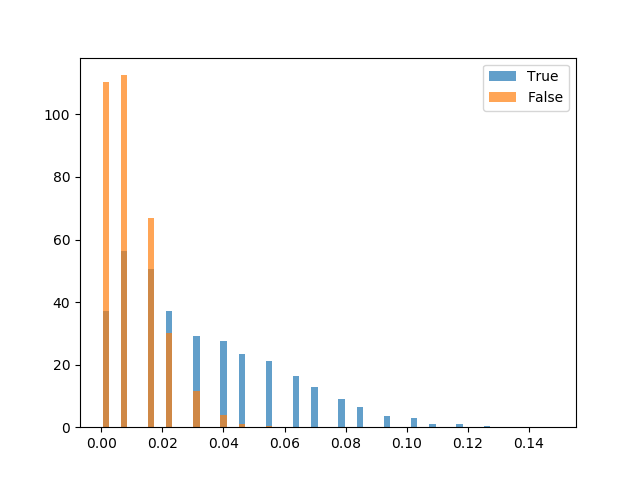
\includegraphics[width = .8\textwidth]{Ecoli_30x_overlap_5000_1000_cutoff_identity_k_10_perm_128.png}
	\caption{Identity for k =10 with 128 permutations}
	\label{fig1}
\end{figure}

\begin{figure}[H]
	\centering
	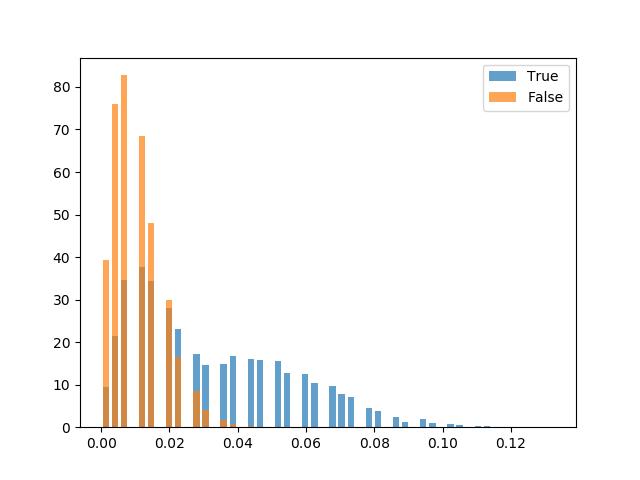
\includegraphics[width = .8\textwidth]{Ecoli_30x_overlap_5000_1000_cutoff_identity_k_10_perm_256.png}
	\caption{Identity for k =10 with 256 permutations}
	\label{fig1}
\end{figure}

\begin{figure}[H]
	\centering
	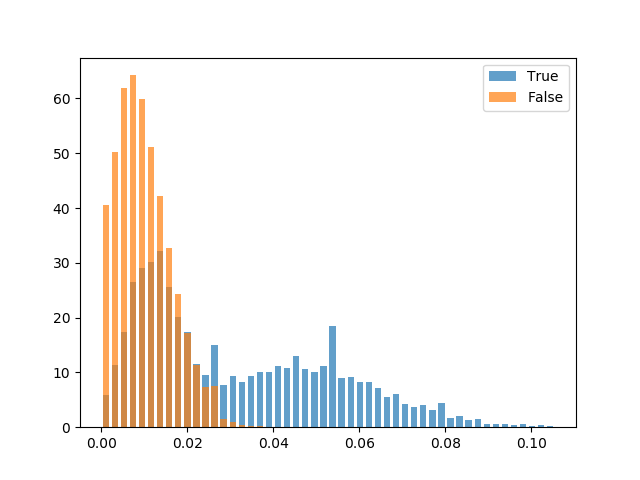
\includegraphics[width = .8\textwidth]{Ecoli_30x_overlap_5000_1000_cutoff_identity_k_10_perm_512.png}
	\caption{Identity for k =10 with 512 permutations}
	\label{fig1}
\end{figure}	
We can see with increasing number of permutations, we have higher resolution to distinguish the true overlap with other non-overlap pair.

The Jaccard similarities are showed below

\begin{figure}[H]
	\centering
	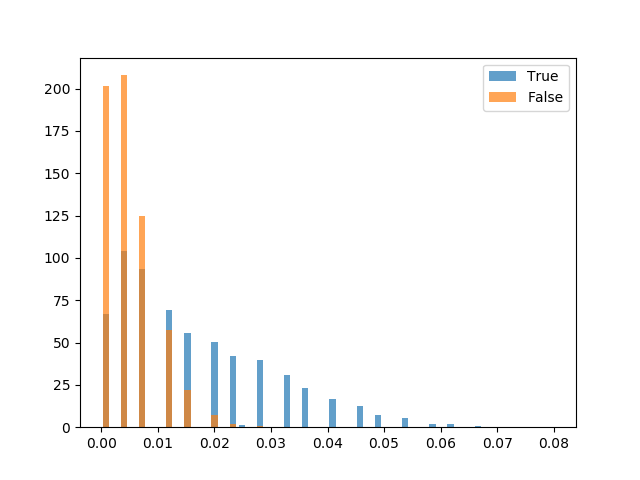
\includegraphics[width = .8\textwidth]{Ecoli_30x_overlap_5000_1000_cutoff_jaccard_k_10_perm_128.png}
	\caption{Jaccard similarity for k =10 with 128 permutations}
	\label{fig1}
\end{figure}

\begin{figure}[H]
	\centering
	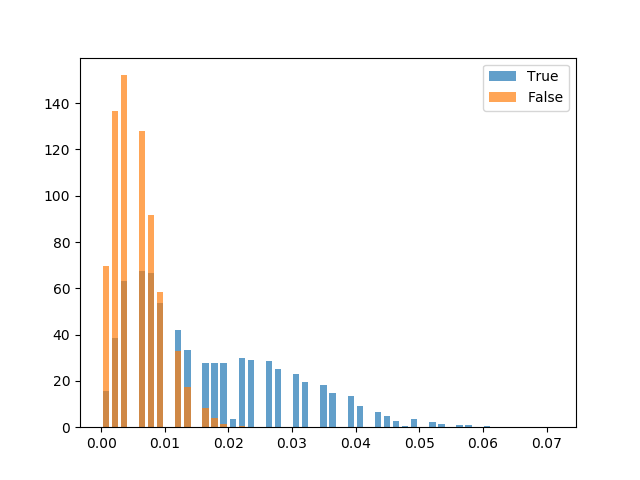
\includegraphics[width = .8\textwidth]{Ecoli_30x_overlap_5000_1000_cutoff_jaccard_k_10_perm_256.png}
	\caption{Jaccard similarity for k =10 with 256 permutations}
	\label{fig1}
\end{figure}

\begin{figure}[H]
	\centering
	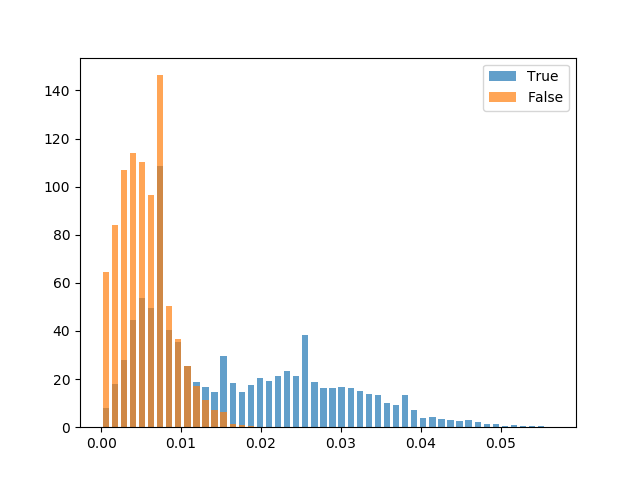
\includegraphics[width = .8\textwidth]{Ecoli_30x_overlap_5000_1000_cutoff_jaccard_k_10_perm_512.png}
	\caption{Jaccard similarity for k =10 with 512 permutations}
	\label{fig1}
\end{figure}
From these figures, we can found that Jaccard similarity is lower than identities.

I also test the size k impact
\begin{figure}[H]
	\centering
	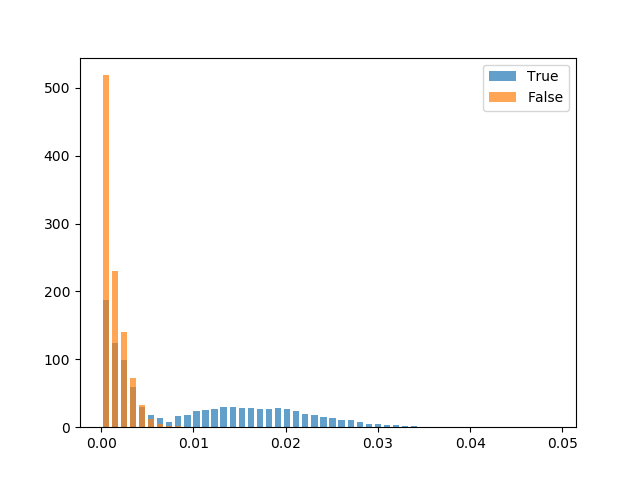
\includegraphics[width = .8\textwidth]{Ecoli_30x_overlap_5000_1000_cutoff_jaccard_k_11_perm_512.png}
	\caption{Identity for k =11 with 512 permutations}
	\label{fig1}
\end{figure}

\begin{figure}[H]
	\centering
	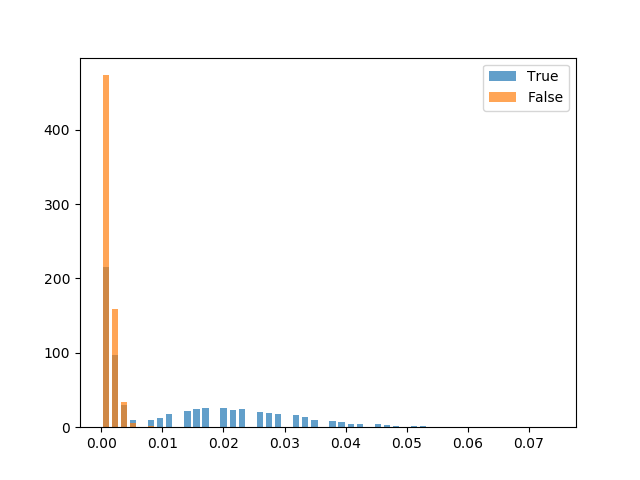
\includegraphics[width = .8\textwidth]{Ecoli_30x_overlap_5000_1000_cutoff_identity_k_12_perm_512.png}
	\caption{Identity for k =12 with 512 permutations}
	\label{fig1}

\end{figure}

With large k, the threshold to distinguish the true and false become less.

I will choose original LSH which should be close to identity.

\part{b}

The false positive rate is given by:
\[ FP = \int_{0}^{s}1 - (1-s^{r})^{b} \]

The false negative rate is given by:
\[ FN = \int_{s}^{1}1- (1 - (1-s^{r})^{b}) \]

I decide to use $ k = 12 $ and $ s = 0.01 $, the optimized $ b = 166 $ and$  r = 1 $ which  minimize the sum of FP and FN. The estimated FN = 1.1239e-05 and estimated FP = 0

\part{c}
I follow the identity and will compare under same band.
LSH hashing function I used is byteswap function from numpy library. Following the optimized b and r, if we can hashing the size r vector from two different read under the same band to one bucket, we will report these two reads as one overlap pair.

\part{e}
Using $ k = 12 $ with 512 permutations and threshold $ = 0.01 $, I got the following result:

sensitivity 0.32540324499214923


FPR 0.3302799701435846


accuracy 0.04372734189679094


F1 0.07709477054188414


Filtration Rate: 0.33006366980337704

The false positive rate obviously much larger than our theory result, I believe this is caused by high error rates of our DNA reads

\part{f}

Because we artificially construct 5000 overlap size threshold, so we can see that a lot of "false positive" are reposted because they just below 5000 threshold.

Noticed here I only count all the pairs that can found overlap sizes.

\begin{figure}[H]
	\centering
	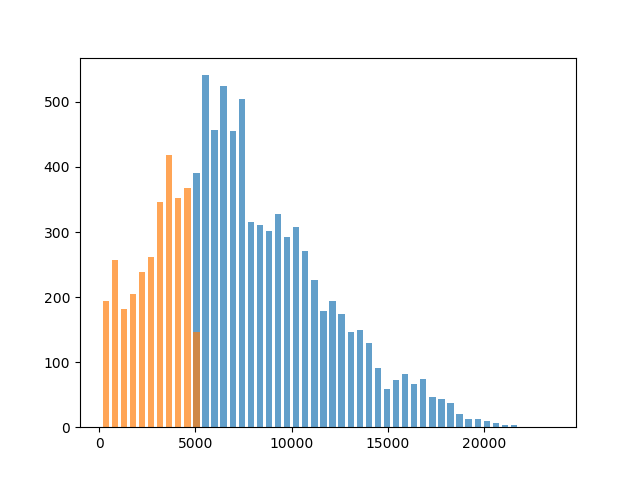
\includegraphics[width = .8\textwidth]{Ecoli_Pacbio_simulate_30X_5000_1000_k12_512_0p01.png}
	\caption{Overlap size comparison of true positive (blue) and false positive (orange)}
	\label{fig1}
	
\end{figure}


\question{3}{}
I use k = 10 with 1024 permutations and 0.04 threshold. Optimized $ b = 512 $ and $ r = 2 $, respectively


Total pairs: 233586.0, Expected Overlap: 22220, Total report: 35765, True Positive: 4094

sensitivity 0.18424842484248424

FPR 0.1498396146967819

accuracy 0.11446945337620579

F1 0.14120893334483056

Filtration Rate: 0.15311277216956495

\question{4}{}

I plot the number of corrected clusters against size of that cluster.

With larger k, we can see we have more clusters and there are more and more correct clusters. And in general, the larger cluster tends to has error.

\begin{figure}[H]
	\centering
	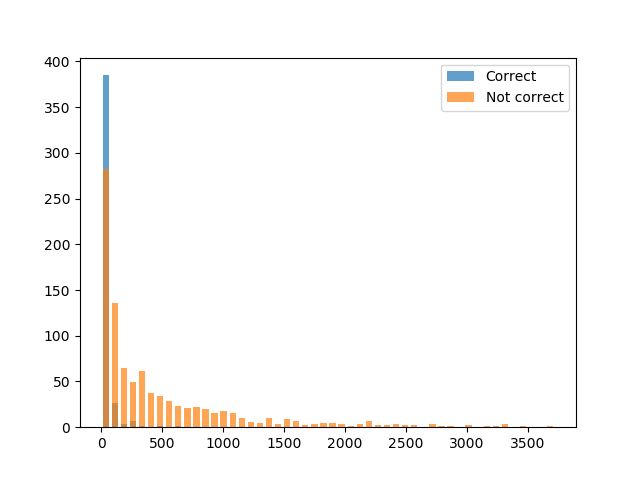
\includegraphics[width = .8\textwidth]{virus_reads_k6_32_cluster.png}
	\caption{Number of clusters against cluster size with k = 6 and permutation = 32}
	\label{fig1}	
\end{figure}

\begin{figure}[H]
	\centering
	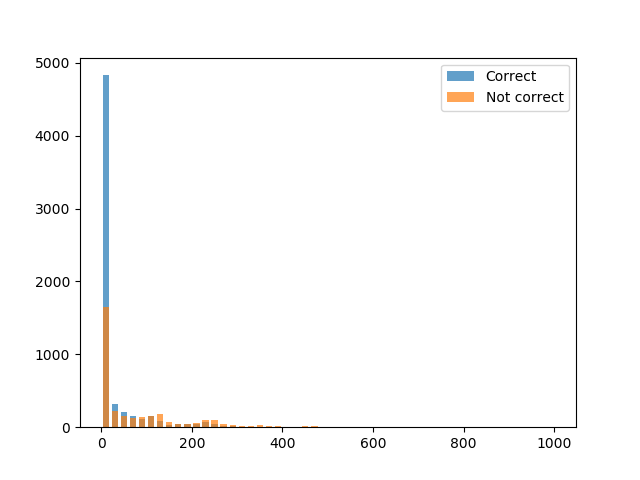
\includegraphics[width = .8\textwidth]{virus_reads_k8_32_cluster.png}
	\caption{Number of clusters against cluster size with k = 8 and permutation = 32}
	\label{fig1}	
\end{figure}

\begin{figure}[H]
	\centering
	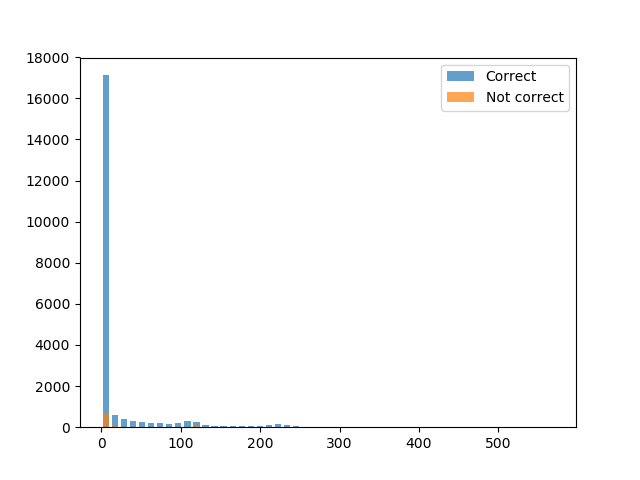
\includegraphics[width = .8\textwidth]{virus_reads_k10_32_cluster.png}
	\caption{Number of clusters against cluster size with k = 10 and permutation = 32}
	\label{fig1}	
\end{figure}

\begin{figure}[H]
	\centering
	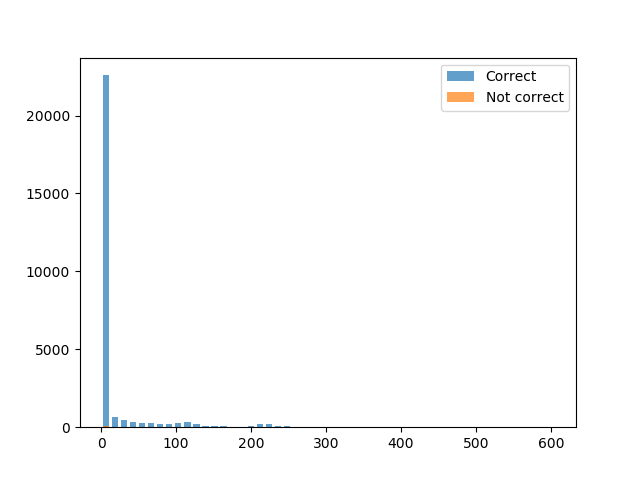
\includegraphics[width = .8\textwidth]{virus_reads_k12_32_cluster.png}
	\caption{Number of clusters against cluster size with k = 12 and permutation = 32}
	\label{fig1}	
\end{figure}

\begin{figure}[H]
	\centering
	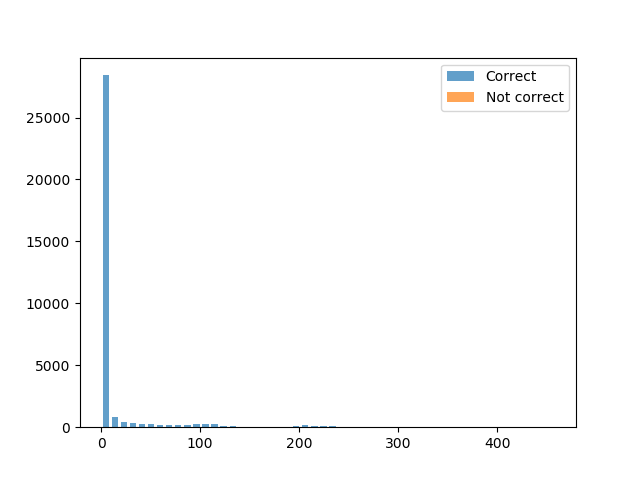
\includegraphics[width = .8\textwidth]{virus_reads_k16_32_cluster.png}
	\caption{Number of clusters against cluster size with k = 16 and permutation = 32}
	\label{fig1}	
\end{figure}

\end{document}
